% =====================================================================
\lecture{3}{חומר אפל והרשת הקוסמית: הפרעות לינאריות ואורך ג'ינס}{מפגש 2, כשעה ורבע. \ (5' הבעיה, 20' גזירה ניוטונית, 25' \en{GR} ופתרונות מעל האופק, 5' רשת קוסמית, תרגילים)}
% =====================================================================

\begin{goalbox}
\textbf{מטרות.} (1) לגזור את משוואת הצמיחה הלינארית מהידרודינמיקה ניוטונית ביקום מתפשט. (2) לקבל ממנה את אורך ג'ינס ולהבין למה בריונים לבדם לא מספיקים. (3) לגזור את ההפרעות מ-\en{GR} בכיול הניוטוני, להראות שמתקבלת אותה משוואת צמיחה בדיוק (לצפיפות הקומובילית), ולפתור מעל האופק בעידני החומר והקרינה. (4) ממבנה לינארי לרשת: \en{Zel'dovich} וקריסה כדורית.
\end{goalbox}

\subsection{הבעיה}
ב-\en{CMB}: $\delta T/T\sim10^{-5}$, ולכן $\delta\equiv\delta\rho/\bar\rho\sim10^{-5}$ ב-$z\approx1100$. היום: גלקסיות עם $\delta\sim10^{6}$ וצבירים עם $\delta\sim200$. איך צומחים פקטור $\gtrsim10^5$?

\subsection{גזירה ניוטונית}
\textbf{משוואות.} רציפות, אוילר ופואסון לנוזל עם צפיפות $\rho$, מהירות $\mathbf V$, לחץ $p$:
\begin{equation}
\partial_t\rho+\nabla\!\cdot(\rho\mathbf V)=0,\qquad
\partial_t\mathbf V+(\mathbf V\!\cdot\!\nabla)\mathbf V=-\nabla\Phi-\frac{\nabla p}{\rho},\qquad
\nabla^2\Phi=4\pi G\rho .
\end{equation}
\textbf{רקע.} $\rho=\bar\rho(t)$, $\mathbf V=H\mathbf r$. רציפות: $\bar\rho\propto a^{-3}$. אוילר ופואסון: $\ddot a/a=-\tfrac{4\pi G}{3}\bar\rho$ --- משוואת פרידמן לחומר. \emph{הרקע הוא יקום פרידמן; לא הנחנו זאת.}

\begin{warnbox}
\textbf{ג'ינס במדיום סטטי} (1902): $\nabla^2\Phi_0=4\pi G\rho_0\neq0$ עם $\Phi_0=$ קבוע --- סתירה, שג'ינס "התעלם" ממנה (\en{Jeans swindle}). ביקום מתפשט אין סתירה: $\Phi_0=-\tfrac12(\ddot a/a)r^2$ פותר את פואסון. ההתפשטות היא שמצדיקה את החישוב.
\end{warnbox}

\textbf{הפרעות.} $\rho=\bar\rho(1+\delta)$, $\mathbf V=H\mathbf r+\mathbf u$, $\Phi=\Phi_0+\phi$, $\delta p=c_s^2\bar\rho\delta$. בקואורדינטות נעות $\mathbf x=\mathbf r/a$ (אז $\nabla_r=a^{-1}\nabla_x$), סדר ראשון:
\begin{equation}
\dot\delta+\frac1a\nabla\!\cdot\mathbf u=0,\qquad
\dot{\mathbf u}+H\mathbf u=-\frac1a\nabla\phi-\frac{c_s^2}{a}\nabla\delta,\qquad
\nabla^2\phi=4\pi G\bar\rho a^2\delta .
\end{equation}
האיבר $H\mathbf u$ הוא "חיכוך האבל": בלי כוחות $\mathbf u\propto1/a$. נגזרת זמן של הראשונה, דיברגנץ של השנייה, הצבה, ומעבר לפורייה ($\nabla^2\to-k^2$, $k$ נע):
\begin{equation}
\boxed{\;\ddot\delta_k+2H\dot\delta_k=\Big(4\pi G\bar\rho-\frac{c_s^2k^2}{a^2}\Big)\delta_k\;}
\label{eq:growth}
\end{equation}
מתנד מרוסן שבו "קבוע הקפיץ" מחליף סימן. כל מוד $k$ מתפתח בנפרד --- רק בתורה הלינארית.

\subsection{אורך ג'ינס}
הכבידה מנצחת את הלחץ כאשר $k<k_J$:
\begin{equation}
\boxed{\;k_J=\frac{a\sqrt{4\pi G\bar\rho}}{c_s},\qquad
\lambda_J=\frac{2\pi a}{k_J}=c_s\sqrt{\frac{\pi}{G\bar\rho}},\qquad
M_J=\frac{4\pi}{3}\bar\rho\Big(\frac{\lambda_J}{2}\Big)^3\;}
\end{equation}
\begin{itemize}
\item $\lambda>\lambda_J$: צמיחה. \quad $\lambda<\lambda_J$: גלי קול (תנודות אקוסטיות --- הבסיס של הרצאה 5).
\item פיזיקלית: $\lambda_J\sim c_s\,t_{\rm ff}$ --- המרחק שגל קול עובר בזמן נפילה חופשית $t_{\rm ff}\sim(G\rho)^{-1/2}$.
\end{itemize}

\begin{figure}[htbp]\centering
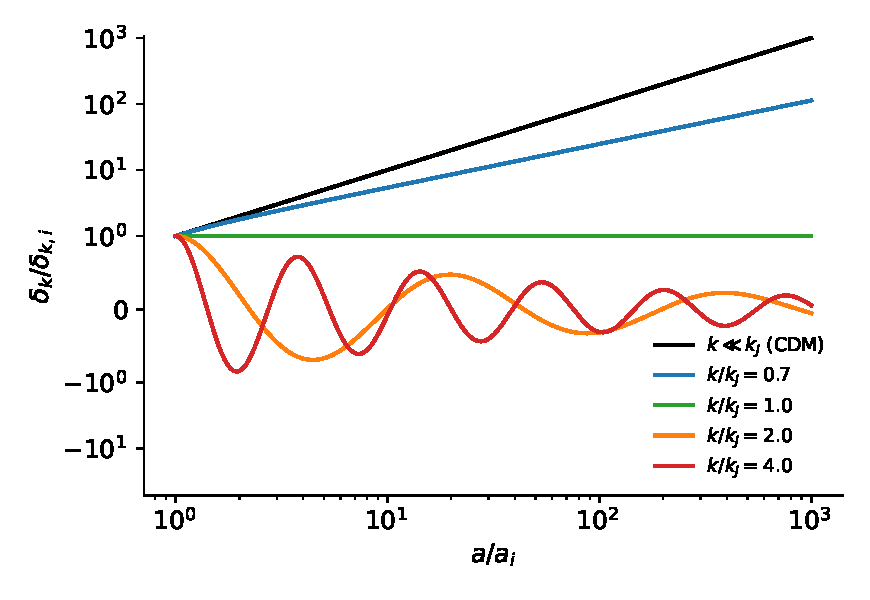
\includegraphics[width=0.55\textwidth]{figs/fig_jeans.pdf}
\caption{\small פתרון נומרי של \eqref{eq:growth} ב-\en{EdS} עבור יחס קבוע $k/k_J$. מתחת ל-$k_J$ ההפרעה צומחת; מעליו היא מתנודדת ודועכת.}
\end{figure}

\subsection{פתרונות, ולמה צריך חומר אפל}
\begin{keybox}
\textbf{\en{EdS}, $c_s=0$:} $4\pi G\bar\rho=\frac{2}{3t^2}$, $H=\frac{2}{3t}$. הצבת $\delta\propto t^n$: $3n^2+n-2=0$, ולכן
\begin{equation}
\delta_+\propto t^{2/3}\propto a,\qquad \delta_-\propto t^{-1}.
\end{equation}
הצמיחה היא \emph{חזקה} של $a$, לא מעריכית. ב-$\Lambda$: $\bar\rho\to0$ ו-$\delta\to$ קבוע. בעידן הקרינה (מתחת לאופק): $\delta_m\propto\ln a$ (\en{Mészáros}) --- הקרינה מגדילה את $H$ אבל לא מתקבצת.
\end{keybox}
\textbf{הטיעון.} בריונים צמודים לפוטונים עד $z\approx1100$: $c_s\approx c/\sqrt3$ ו-$M_J\sim10^{17}\Msun$, יותר ממסת האופק (תרגיל 3.1). הם מתחילים לצמוח רק ב-$z\approx1100$, ועד היום מקבלים פקטור $\lesssim1100$:
\begin{equation}
10^{-5}\times10^{3}=10^{-2}\ll1 .
\end{equation}
\emph{לא היו גלקסיות.} חומר שאינו מצומד לפוטונים צומח כבר מ-$z_{\rm eq}\approx3400$ (ולוגריתמית לפני כן), ואחרי הרקומבינציה הבריונים נופלים לבורות מוכנים.

\textbf{חם או קר?} חלקיקים מהירים זורמים החוצה מבורות (\en{free streaming}): בסולמות מתחת ל-$\lambda_{\rm fs}\sim\int v\,dt/a$ ההפרעות נמחקות. לנייטרינו ($m\sim\mathrm{eV}$) $\lambda_{\rm fs}\sim100\,\Mpc$: מבנה גדול נוצר ראשון ומתפרק (\en{top-down}), בניגוד לתצפית שגלקסיות זקנות מצבירים. לכן החומר האפל \textbf{קר}: $v\ll c$ מאז ההתנתקות, מבנה נבנה מלמטה למעלה (\en{bottom-up}).

\textbf{קצב הצמיחה.} $f\equiv d\ln D/d\ln a\simeq\Omega_m(a)^{0.55}$ ב-\en{GR}. נמדד מעיוותי מרחב-הסחה (\en{RSD}) כ-$f\sigma_8$, מבחן ישיר לכבידה.

\subsection{הגזירה היחסותית: מהמטריקה ועד משוואת הצמיחה}
הגזירה הניוטונית הניחה פואסון ומהירויות קטנות. כאן לא מניחים כבידה ניוטונית: מפריעים את \emph{המטריקה}, מחשבים את העקמומיות, ומשווים ל-$T^\mu{}_\nu$, בדיוק כמו בגזירת משוואות פרידמן בהרצאה 1. החשבון ארוך, אבל לכל רכיב של המשוואות יש תפקיד אחד:
\begin{center}\small
\begin{tabular}{@{}lll@{}}
\toprule
משוואה & סוג & מה היא נותנת \\ \midrule
רכיב $00$ של איינשטיין & אילוץ & פואסון יחסותי: $\Phi\leftrightarrow\delta$ \\
רכיב $0i$ & אילוץ & $\Phi'\leftrightarrow$ זרימת החומר $\theta$ \\
רכיב $ij$ חסר עקבה & אילוץ & $\Phi=\Psi$ \\
רכיב $ij$ עקבה & דינמי & התפתחות $\Phi$ (לא עצמאי כשיש רק אבק) \\
$\nabla_\mu T^\mu{}_0=0$ & שימור & רציפות: התפתחות $\delta$ \\
$\nabla_\mu T^\mu{}_i=0$ & שימור & אוילר: התפתחות $\theta$ \\ \bottomrule
\end{tabular}
\end{center}

\textbf{שלב 0: הרקע בזמן קונפורמי.} $d\eta=dt/a$, $ds^2=a^2(\eta)(-d\eta^2+d\mathbf x^2)$, $'\equiv d/d\eta$, $\mathcal H\equiv a'/a=aH$. משוואות פרידמן (שטוח) הופכות ל-
\begin{equation}
\begin{gathered}
\mathcal H^2=\frac{8\pi G}{3}a^2\rho,\qquad \mathcal H'=-\frac{4\pi G}{3}a^2(\rho+3p),\qquad \rho'=-3\mathcal H(\rho+p),\\
\Rightarrow\qquad \mathcal H^2-\mathcal H'=4\pi Ga^2(\rho+p).
\end{gathered}
\label{eq:gr-bg}
\end{equation}
($\Lambda$ היא נוזל עם $p=-\rho$, ולכן לא תורמת ל-$\rho+p$.) בעידן החומר $a\propto\eta^2$, $\mathcal H=2/\eta$; בעידן הקרינה $a\propto\eta$, $\mathcal H=1/\eta$.

\textbf{שלב 1: המטריקה המופרעת וחופש הכיול.} להפרעה כללית יש חלקים סקלריים (קשורים לצפיפות), וקטוריים (דועכים) וטנזוריים (גלי כבידה, הרצאה 6), שבסדר ראשון אינם מתערבבים. לחלק הסקלרי ארבע פונקציות, אבל טרנספורמציית קואורדינטות $x^\mu\to x^\mu+\xi^\mu$ (שתי פונקציות סקלריות) מסלקת שתיים. הבחירה הנוחה היא \textbf{הכיול הניוטוני}:
\begin{equation}
\boxed{\;ds^2=a^2(\eta)\big[-(1+2\Psi)\,d\eta^2+(1-2\Phi)\,\delta_{ij}dx^idx^j\big]\;},\qquad|\Phi|,|\Psi|\ll1 .
\end{equation}
$\Psi$ משנה את קצב השעון המקומי (הפוטנציאל הניוטוני); $\Phi$ משנה את העקמומיות המרחבית. ב-\en{CMB} $|\Phi|\sim10^{-5}$.

\begin{warnbox}
\textbf{$\delta$ תלויה בכיול.} שינוי כיול מזיז את משטחי $t=$ קבוע, ולכן משנה את $\delta\rho/\rho$ באיבר מסדר $3\mathcal H\theta/k^2$. מתחת לאופק ($k\gg\mathcal H$) זה זניח; מעל האופק זה מכריע. לכן מעל האופק צריך לבחור גודל שאינו תלוי בכיול (להלן: $\Delta$ ו-$\mathcal R$).
\end{warnbox}

\textbf{שלב 2: סמלי כריסטופל} (סדר ראשון; אפס הסדר הוא של הרצאה 1):
\begin{align}
\Gamma^0_{00}&=\mathcal H+\Psi', & \Gamma^0_{0i}&=\Gamma^i_{00}=\partial_i\Psi, & \Gamma^0_{ij}&=\big[\mathcal H-2\mathcal H(\Phi+\Psi)-\Phi'\big]\delta_{ij},\notag\\
\Gamma^i_{0j}&=(\mathcal H-\Phi')\,\delta^i_j, & \Gamma^i_{jk}&=-\big(\delta^i_j\partial_k\Phi+\delta^i_k\partial_j\Phi-\delta_{jk}\partial_i\Phi\big). &&
\end{align}
למשל $\Gamma^0_{ij}=-\tfrac12g^{00}\partial_0g_{ij}=(1-2\Psi)\big[\mathcal H(1-2\Phi)-\Phi'\big]\delta_{ij}$. ההפרעה מוסיפה רק נגזרות זמן של הפוטנציאלים ו"כוחות" (גרדיאנטים).

\textbf{שלב 3: העקמומיות.} מציבים בטנזור ריצ'י ומרכיבים $G^\mu{}_\nu$ (חשבון ארוך; כדאי לבדוק סימבולית):
\begin{align}
a^2\,\delta G^0{}_0&=-2\nabla^2\Phi+6\mathcal H(\Phi'+\mathcal H\Psi),\notag\\
a^2\,\delta G^0{}_i&=-2\,\partial_i(\Phi'+\mathcal H\Psi),\notag\\
a^2\,\delta G^i{}_j&=\delta^i_j\big[2\Phi''+2\mathcal H(\Psi'+2\Phi')+2(2\mathcal H'+\mathcal H^2)\Psi+\nabla^2(\Psi-\Phi)\big]+\partial_i\partial_j(\Phi-\Psi).
\end{align}
ב-$\delta G^0{}_0$ וב-$\delta G^0{}_i$ אין נגזרות זמן שניות: אלה אילוצים, כמו משוואת פרידמן הראשונה. רק $\delta G^i{}_j$ דינמי, והחלק $\partial_i\partial_j(\Phi-\Psi)$ שלו חסר עקבה.

\textbf{שלב 4: החומר.} נוזל מושלם $T^\mu{}_\nu=(\rho+p)u^\mu u_\nu+p\delta^\mu_\nu$ עם $\rho\to\rho(1+\delta)$, $p\to p+\delta p$ ו-$v^i=dx^i/d\eta$ (זו בדיוק המהירות הפקוליארית $\mathbf u$ של הגזירה הניוטונית, כי $a\,dx/dt=dx/d\eta$). מהנרמול $u^\mu u_\mu=-1$: $u^\mu=a^{-1}(1-\Psi,\,v^i)$, ולכן
\begin{equation}
T^0{}_0=-\rho(1+\delta),\qquad T^0{}_i=(\rho+p)v_i,\qquad T^i{}_j=(p+\delta p)\,\delta^i_j .
\end{equation}
להפרעות סקלריות $v_i=\partial_iv$, ומשתמשים בדיברגנץ $\theta\equiv\nabla\!\cdot\mathbf v$.

\textbf{שלב 5: שימור --- רציפות ואוילר יחסותיות.} משוואות החומר נובעות מ-$\nabla_\mu T^\mu{}_\nu=0$, עם $\Gamma^\mu_{\mu0}=4\mathcal H+\Psi'-3\Phi'$ ו-$\Gamma^\mu_{\mu i}=\partial_i(\Psi-3\Phi)$. אחרי הורדת אפס הסדר ($\rho'=-3\mathcal H(\rho+p)$), ל-$w$ ו-$c_s^2=\delta p/\delta\rho$ קבועים:
\begin{equation}
\boxed{\;\delta'=-(1+w)(\theta-3\Phi')-3\mathcal H(c_s^2-w)\,\delta,\qquad
\theta'+\mathcal H(1-3w)\theta=k^2\Psi+\frac{c_s^2k^2}{1+w}\delta\;}
\label{eq:gr-fluid}
\end{equation}
(אוילר בפורייה, $\nabla^2\to-k^2$.) לאבק: $\delta'=-\theta+3\Phi'$ ו-$\theta'+\mathcal H\theta=k^2\Psi$. זו הגרסה הניוטונית ($\dot\delta=-\theta/a$, $\dot{\mathbf u}+H\mathbf u=-\nabla\phi/a$) עם תוספת אחת: $3\Phi'$, השינוי בנפח המקומי כשהעקמומיות המרחבית משתנה. הרוטור של אוילר נותן $\omega\propto a^{-(1-3w)}$: מערבולות דועכות, ולכן מספיק לטפל בחלק הסקלרי.

\textbf{שלב 6: משוואות איינשטיין, רכיב אחר רכיב} ($\delta G^\mu{}_\nu=8\pi G\,\delta T^\mu{}_\nu$, בפורייה):
\begin{align}
(00)\quad& k^2\Phi+3\mathcal H(\Phi'+\mathcal H\Psi)=-4\pi Ga^2\rho\,\delta, \label{eq:gr-00}\\
(0i)\quad& k^2(\Phi'+\mathcal H\Psi)=4\pi Ga^2(\rho+p)\,\theta, \label{eq:gr-0i}\\
(ij,\ \text{חסר עקבה})\quad& \Phi-\Psi=0, \label{eq:gr-slip}\\
(ij,\ \text{עקבה})\quad& \Phi''+\mathcal H(\Psi'+2\Phi')+(2\mathcal H'+\mathcal H^2)\Psi=4\pi Ga^2\,\delta p . \label{eq:gr-ii}
\end{align}

\begin{keybox}
\textbf{שני פוטנציאלים, ולמה הם שווים.} את החלק חסר העקבה מזין רק מאמץ אניזוטרופי (בעיקר נייטרינו חופשיים, תיקון של כ-10\% בעידן הקרינה). לנוזל מושלם $\Phi=\Psi$. חלקיק איטי מרגיש את $\Psi$ ואור מרגיש את $\Phi+\Psi$; בתורות כבידה מתוקנות לרוב $\Phi\ne\Psi$, ולכן השוואת עדשות כבידה למהירויות גלקסיות היא מבחן ישיר של \en{GR}.
\end{keybox}

\textbf{פואסון מדויק.} מציבים את (0i) ב-(00) ומגדירים את הצפיפות הקומובילית (הניגוד במערכת שנעה עם החומר):
\begin{equation}
\Delta\equiv\delta+\frac{3\mathcal H(1+w)}{k^2}\,\theta\qquad\Longrightarrow\qquad
\boxed{\;k^2\Phi=-4\pi Ga^2\rho\,\Delta\;}
\label{eq:gr-poisson}
\end{equation}
זה פואסון \emph{בדיוק}, בכל סולם. מתחת לאופק $\Delta\simeq\delta$, וזו ההצדקה לפואסון של הגזירה הניוטונית.

\textbf{שלב 7: משוואת הצמיחה, מדויקת.} לאבק על רקע שטוח של חומר ו-$\Lambda$ חלקה: $\mathcal H^2-\mathcal H'=4\pi Ga^2\rho_m$ \eqref{eq:gr-bg}. גוזרים את $\Delta=\delta+3\mathcal H\theta/k^2$ ומציבים את \eqref{eq:gr-fluid}:
\begin{equation}
\Delta'=-\theta+3(\Phi'+\mathcal H\Phi)+\frac{3(\mathcal H'-\mathcal H^2)}{k^2}\theta .
\end{equation}
לפי (0i) $3(\Phi'+\mathcal H\Phi)=12\pi Ga^2\rho_m\theta/k^2$, ולפי הרקע $3(\mathcal H'-\mathcal H^2)=-12\pi Ga^2\rho_m$: שני האיברים מתבטלים \emph{בדיוק}, ו-$\Delta'=-\theta$. גזירה נוספת עם אוילר ופואסון:
$\Delta''=-\theta'=\mathcal H\theta-k^2\Phi=-\mathcal H\Delta'+4\pi Ga^2\rho_m\Delta$, כלומר
\begin{equation}
\boxed{\;\Delta''+\mathcal H\Delta'=4\pi Ga^2\rho_m\Delta\quad\Longleftrightarrow\quad\ddot\Delta+2H\dot\Delta=4\pi G\bar\rho_m\Delta\;}
\label{eq:gr-growth}
\end{equation}
(עם $\Delta'=a\dot\Delta$, $\Delta''=a^2(\ddot\Delta+H\dot\Delta)$.) זו משוואה \eqref{eq:growth} עם $c_s=0$, אבל עכשיו היא נכונה \emph{בכל הסולמות, גם מעל האופק}, עבור $\Delta$. מתחת לאופק, למוד הגדל ($\theta=-\mathcal Hf\Delta$), $\delta=\Delta(1+3f\mathcal H^2/k^2)$: התיקון קטן מ-$10^{-4}$ לכל $k>0.1\,h\,\Mpc^{-1}$ היום.

\subsection{פתרונות יחסותיים: מה קורה מעל האופק}
\textbf{עידן החומר.} $w=\delta p=0$, $\mathcal H=2/\eta$, ולכן $2\mathcal H'+\mathcal H^2=0$ ו-\eqref{eq:gr-ii} הופכת ל-$\Phi''+\frac6\eta\Phi'=0$:
\begin{equation}
\Phi=C_1+C_2\,\eta^{-5}\quad\Longrightarrow\quad\boxed{\Phi=\text{קבוע בכל הסולמות}} .
\end{equation}
מפואסון \eqref{eq:gr-poisson} עם $4\pi Ga^2\rho=\tfrac32\mathcal H^2=6/\eta^2$: $\Delta=-\frac{k^2\eta^2}{6}\Phi\propto a$, כמו בפתרון הניוטוני. ומ-(00) עם $\Phi'=0$:
\begin{equation}
\delta=-2\Phi-\frac{2k^2}{3\mathcal H^2}\Phi=
\begin{cases}-2\Phi=\text{קבוע}, & k\ll\mathcal H\ \ (\text{מעל האופק})\\[2pt] \Delta\propto a, & k\gg\mathcal H\ \ (\text{מתחת לאופק})\end{cases}
\end{equation}
בכיול הניוטוני $\delta$ "קפואה" מעל האופק, אבל זה אפקט כיול: $\Delta$ צומח כ-$a$ בכל סולם. אזור צפוף ($\delta>0$) הוא בור פוטנציאל ($\Phi<0$). המהירות מ-(0i): $\theta=\frac{2k^2}{3\mathcal H}\Phi$.

\textbf{עידן הקרינה.} $w=c_s^2=\tfrac13$, $\mathcal H=1/\eta$. משלבים את העקבה \eqref{eq:gr-ii} (עם $\delta p=\tfrac13\rho\delta$) עם (00) ומקבלים משוואה סגורה ל-$\Phi$:
\begin{equation}
\Phi''+\frac4\eta\Phi'+\frac{k^2}{3}\Phi=0\quad\Longrightarrow\quad
\Phi=3\Phi_p\,\frac{\sin x-x\cos x}{x^3},\qquad x=\frac{k\eta}{\sqrt3}=k\,r_s .
\end{equation}
מעל אופק הקול ($x\ll1$): $\Phi\to\Phi_p$, קבוע. מתחת לו: $\Phi$ מתנודד ודועך כ-$x^{-2}\propto a^{-2}$, כי לחץ הקרינה מונע התקבצות. זה מקור תנודות ה-\en{CMB} (הרצאה 5) ומקור אפקט \en{Mészáros}: חומר אפל שנכנס לאופק בעידן הקרינה מאבד את הפוטנציאל שדחף אותו, ולכן גדל רק לוגריתמית.

\begin{keybox}
\textbf{גודל שנשמר: העקמומיות $\mathcal R$.} הגודל $\mathcal R=-\Phi-\frac{2}{3(1+w)}\Big(\frac{\Phi'}{\mathcal H}+\Phi\Big)$ קבוע מעל האופק לכל $w$ (גם במעברים). עם $\Phi$ קבוע: $\mathcal R=-\frac{5+3w}{3+3w}\Phi$, כלומר $-\tfrac32\Phi$ בקרינה ו-$-\tfrac53\Phi$ בחומר. מכאן
\[\Phi_{\rm MD}=\tfrac{9}{10}\,\Phi_{\rm RD}\qquad(\text{מעל האופק}).\]
$\mathcal R$ הוא מה שאינפלציה קובעת (הרצאה 6), ו-$\Phi$ הוא מה שה-\en{CMB} רואה דרך \en{Sachs--Wolfe}, $\delta T/T=\Phi/3$.
\end{keybox}

\textbf{מה \en{GR} מוסיפה, בסיכום.}
\begin{itemize}
\item משוואת הצמיחה זהה, אבל עבור $\Delta$ ובכל סולם. מתחת ל-$\sim100\,\Mpc$ ובמהירויות $\ll c$ הגישה הניוטונית מדויקת, ולכן סימולציות \en{N}-גופים ניוטוניות עובדות.
\item מעל האופק: $\delta$ תלויה בכיול; $\Phi$ ו-$\mathcal R$ קבועים, והם המחברים בין אינפלציה, \en{CMB} ומבנה.
\item לחץ: $\Phi$ דועך מתחת לאופק בעידן הקרינה. גם $\Lambda$ גורמת ל-$\Phi$ לדעוך (כי $D/a$ יורד), וזה אפקט \en{ISW} ב-\en{CMB}.
\item \en{GR} מנבאת $\Phi=\Psi$, ואור מושפע מ-$\Phi+\Psi$: עדשות כבידה, \en{ISW} וה-\en{CMB} עצמו.
\end{itemize}

\subsection{מלינארי לרשת קוסמית}
\textbf{קירוב \en{Zel'dovich}.} $\mathbf x(\mathbf q,t)=\mathbf q-D(t)\nabla_q\psi(\mathbf q)$. הצפיפות:
\begin{equation}
1+\delta=\frac{1}{(1-D\lambda_1)(1-D\lambda_2)(1-D\lambda_3)},
\end{equation}
כאשר $\lambda_1\ge\lambda_2\ge\lambda_3$ ערכים עצמיים של טנזור העיוות $\partial_i\partial_j\psi$. הציר הראשון קורס ראשון ונוצר \textbf{לוח} (\en{pancake}), אחריו \textbf{פילמנט} (שני צירים), ולבסוף \textbf{צומת} (שלושה). מספר הערכים החיוביים מסווג את הרשת: צמתים, פילמנטים, לוחות וחללים.

\textbf{קריסה כדורית.} קליפה סגורה היא יקום פרידמן קטן עם $k=+1$: מתפשטת, נעצרת (\en{turnaround}) וקורסת. התורה הלינארית הייתה נותנת בקריסה $\delta_c=1.686$; לאחר ויריאליזציה הניגוד האמיתי $\Delta_{\rm vir}=18\pi^2\approx178$ ($\approx200$, מקור "$M_{200}$"; תרגיל 3.3; הגזירה המלאה וההשלכות לחומר אפל בסעיף~\ref{sec:sc}). אחת הדרכים לזהות הילה בסימולציה.

\begin{figure}[htbp]\centering
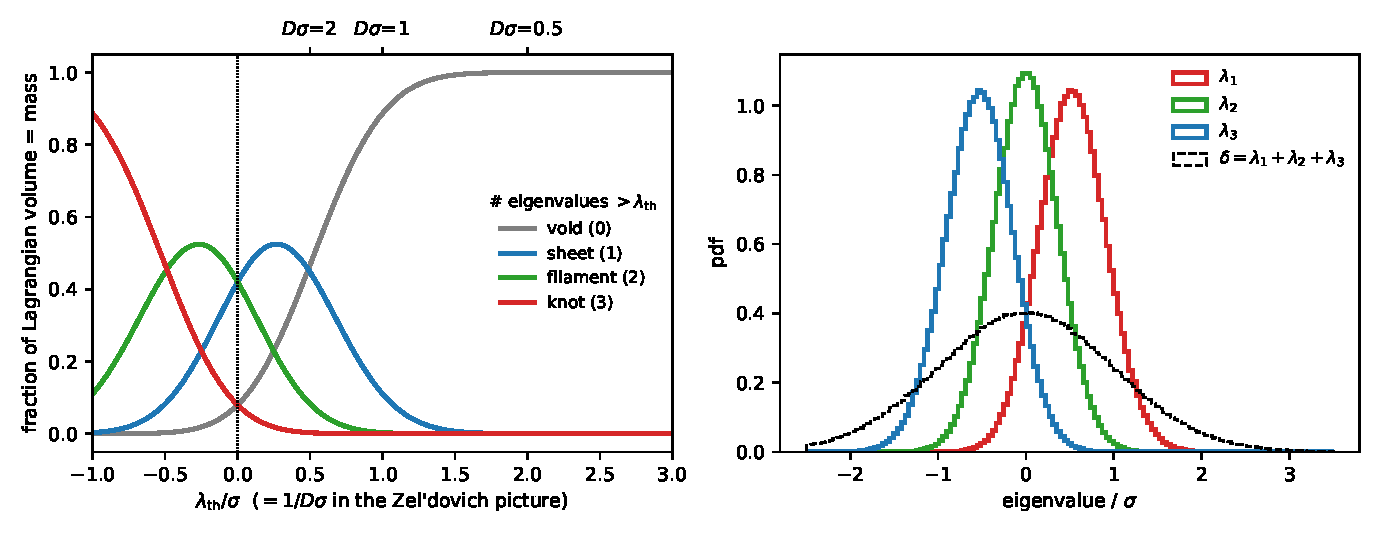
\includegraphics[width=0.85\textwidth]{figs/fig_web_stats.pdf}
\caption{\small סטטיסטיקה של רכיבי הרשת הקוסמית: צמתים, פילמנטים, לוחות וחללים, בנפח ובמסה.}
\end{figure}

% ---------------------------------------------------------------------
\subsection*{תרגילים}
\begin{exercise}{מסת ג'ינס לפני ואחרי הרקומבינציה}
ב-$z=1100$, עם $\Omega_mh^2=0.143$ ו-$\Omega_bh^2=0.0224$: (א) חשבו $\bar\rho_m$ ו-$\bar\rho_b$. (ב) לפני הרקומבינציה $c_s\simeq c/\sqrt{3(1+R)}$, $R\approx0.6$. חשבו $\lambda_J$ ומסת הבריונים $M_J$. (ג) אחרי הרקומבינציה גז מימן-הליום עם $T\approx3000\,\mathrm K$, $\mu=1.22$: $c_s=\sqrt{5k_BT/3\mu m_p}$. חשבו שוב. איזה עצם אסטרופיזיקלי יש לו מסה כזו?
\end{exercise}
\begin{solbox}
\textbf{פתרון.}\ (א) $1101^3=1.335\times10^9$: $\bar\rho_m=3.6\times10^{-18}$, $\bar\rho_b=5.6\times10^{-19}\,\mathrm{kg\,m^{-3}}$.\\
(ב) $c_s=c/\sqrt{4.8}=1.37\times10^5\,\kms$. $\lambda_J=c_s\sqrt{\pi/G\bar\rho_m}\approx0.5\,\Mpc$ פיזיקלי ($\approx560\,\Mpc$ נע). $M_J=\tfrac{4\pi}{3}\bar\rho_b(\lambda_J/2)^3\approx6\times10^{17}\Msun$: יותר מכל צביר. אין צמיחה בריונית.\\
(ג) $c_s=\sqrt{5k_BT/3\mu m_p}=5.8\,\kms$, $\lambda_J\approx22\,\mathrm{pc}$, $M_J\approx4\times10^4\Msun$: מסה של צביר כדורי. ירידה בפקטור $10^{13}$ בבת אחת.
\end{solbox}

\begin{exercise}{פתרונות הצמיחה}
(א) הראו ש-$\delta\propto t^{2/3}$ ו-$t^{-1}$ פותרים את \eqref{eq:growth} ב-\en{EdS} עם $c_s=0$. (ב) הראו שבמשתנה $\ln a$ המשוואה היא $\delta''+\tfrac12\delta'-\tfrac32\delta=0$. (ג) ביקום של $\Lambda$ בלבד ($H=$ קבוע, $\bar\rho_m\to0$), פתרו והראו ש-$\delta\to$ קבוע. מה זה אומר על מבנה בעתיד?
\end{exercise}
\begin{solbox}
\textbf{פתרון.}\ (א) $\delta=t^n$: $n(n-1)+\tfrac43n-\tfrac23=0\Rightarrow3n^2+n-2=0\Rightarrow n=\tfrac23,\,-1$.\\
(ב) $\frac{d}{dt}=H\frac{d}{d\ln a}$, $\ddot\delta=H^2\delta''+\dot H\delta'$, $\dot H=-\tfrac32H^2$: $H^2(\delta''+\tfrac12\delta')=\tfrac32H^2\delta$. פתרונות $a^1$, $a^{-3/2}$.\\
(ג) $\ddot\delta+2H\dot\delta=0$: $\delta=C_1+C_2e^{-2Ht}\to C_1$. המבנה "קופא": לא ייווצרו צבירים חדשים גדולים יותר.
\end{solbox}

\begin{exercise}{מאיפה $18\pi^2$?}
קליפה כדורית: $R=A(1-\cos\theta)$, $t=B(\theta-\sin\theta)$, עם $A^3=GMB^2$. (א) הראו שב-\en{turnaround} ($\theta=\pi$) הניגוד ביחס לרקע \en{EdS} הוא $1+\delta=9\pi^2/16\approx5.55$. (ב) משפט הוויריאל ושימור אנרגיה נותנים $R_{\rm vir}=R_{\rm ta}/2$, והקריסה ב-$t_{\rm coll}=2t_{\rm ta}$. הראו ש-$\Delta_{\rm vir}=18\pi^2\approx178$.
\end{exercise}
\begin{solbox}
\textbf{פתרון.}\ (א) ב-$\theta=\pi$: $R=2A$, $t=\pi B$. $\rho_{\rm sh}=3M/(32\pi A^3)$, $\bar\rho=1/(6\pi Gt^2)=1/(6\pi^3GB^2)$. היחס: $\frac{18\pi^2GMB^2}{32A^3}=\frac{9\pi^2}{16}$.\\
(ב) ב-$t=2\pi B$ ו-$R=A$: $\rho_{\rm vir}/\bar\rho=\frac{3M}{4\pi A^3}\cdot6\pi G(2\pi B)^2=18\pi^2=178$. (הדרך: $5.55\times2^3\times2^2$; $2^3$ מחצי הרדיוס, $2^2$ מהרקע שדולל בזמן כפול.)
\end{solbox}
